\chapter{Разработка прототипа умного устройства и протокола взаимодействия с использованием 
	белорусской криптографии}

	\section{Поиск существующих имплементаций}
	
	Первой задачей практической части было нахождение существующих реализаций подробно описанных
	выше протоколов с целью дальнейшей работы над криптографическим аспектом этих реализаций.
	В качестве основного протокола для модификаций был выбран протокол ZigBee. Были поставлены
	следующие задачи:
	
	\begin{itemize}
		\item поиск имплементации протокола ZigBee, позволяющей вносить модификации; 
		\item поиск устройств (микроконтроллеров), способных работать на этой имплементации;
		\item изменение или полная замена криптографической составляющей в имплементации.
	\end{itemize}

	К сожалению, открытых реализация оказалось немного. Практически не было найдено библиотек,
	реализующих в полной мере последнюю версию протокола. Проблема заключается в том, что сама
	спецификация находится в закрытом доступе. Для получения спецификации необходимо стать
	членом ZigBee Alliance, что осуществляется на платной основе. Аналогично, все имплементации
	протокола ведущими технологическими компания также являются закрытыми. Это связано с
	коммерческой составляющей, поскольку компании получают прибыль, реализуя устройства
	на собственных прошивках.
	
	По совокупности вышеописанных факторов был выбран другой подход, который не привязан
	к определённому протоколу. Суть данного подхода заключается в самостоятельной реализации
	криптографического уровня защиты и применении его поверх установленного соединения между
	управляющим устройством (хабом) и конечным устройством. В качестве конечного устройства
	в данной работе был выбран прототип умной лампочки.
	
	
	\section{Выбор компонентов и технологий для реализации}
	
	Обновлённые практические задачи были сформулированы следующим образом:
	
	\begin{itemize}
		\item выбор микроконтроллера, который будет служить прототипом умного устройства,
		с возможностью его программирования и прошивки;
		\item установка соединения между управляющим и умным устройствами. Для простоты в качестве
		управляющего устройства в данной работе используется компьютер;
		\item разработка кода (прошивки) для умного устройства (контроллера), а также клиентского
		приложения для управляющего устройства;
		\item реализация защищённого обмена сообщениями с использование белорусского криптографического
		стандарта СТБ 34.101.77.
%		\item модификация стандарта с изменением значения некоторых его параметров;
%		\item оценка стойкости видоизменённого решения.
	\end{itemize}

	В качестве микроконтроллера был выбран ESP8266 (модель NodeMCU V3). Это недорогая модель от
	китайской компании Espressif Systems. Её большим преимуществом является встроенный Wi-Fi модуль. 
	Помимо поддерживаемых протоколов Wi-Fi 802.11 b/g/n и режимов работы как в качестве точки доступа,
	так и клиента, микроконтроллер отличается наличием встроенного стека TCP/IP.
	
	Для программирования данной модели существует широкий выбор языков, платформ и сред, среди
	которых Arduino IDE, Espressif IoT Development Framework (официальный фреймворк от разработчика)
	и многие другие. В данной работе был выбран инструмент PlatformIO \cite{platformio}. Это
	кроссплатформенная интегрированная среда разработки, построенная на основе редактора 
	Visual Studio Code, а также встроенный отладчик, статический анализатор кода и система сборки.
	Платформа поддерживает большое количество микроконтроллеров, среди которых в том числе есть
	ESP8266 NodeMCU. На сайте также представлен широкий выбор библиотек и примеров с кодом.
	Языком разработки на платформе является C++.
	
	При выборе инструментов и технологий для разработки также рассматривались варианты использования
	более высокоуровневых языков программировая, таких как Java \cite{microej} или .NET \cite{nanoFramework}.
	Однако наличие примеров, библиотек и большого сообщества разработчиков стало определяющим
	фактором при выборе PlatformIO. При этом для клиентского веб-приложения на управляющем устройстве
	(компьютере) был выбран язык программирования Java.
	
	
	\section{Работа с микроконтроллером ESP8266}
	
	\begin{figure}[h]
		\centering
		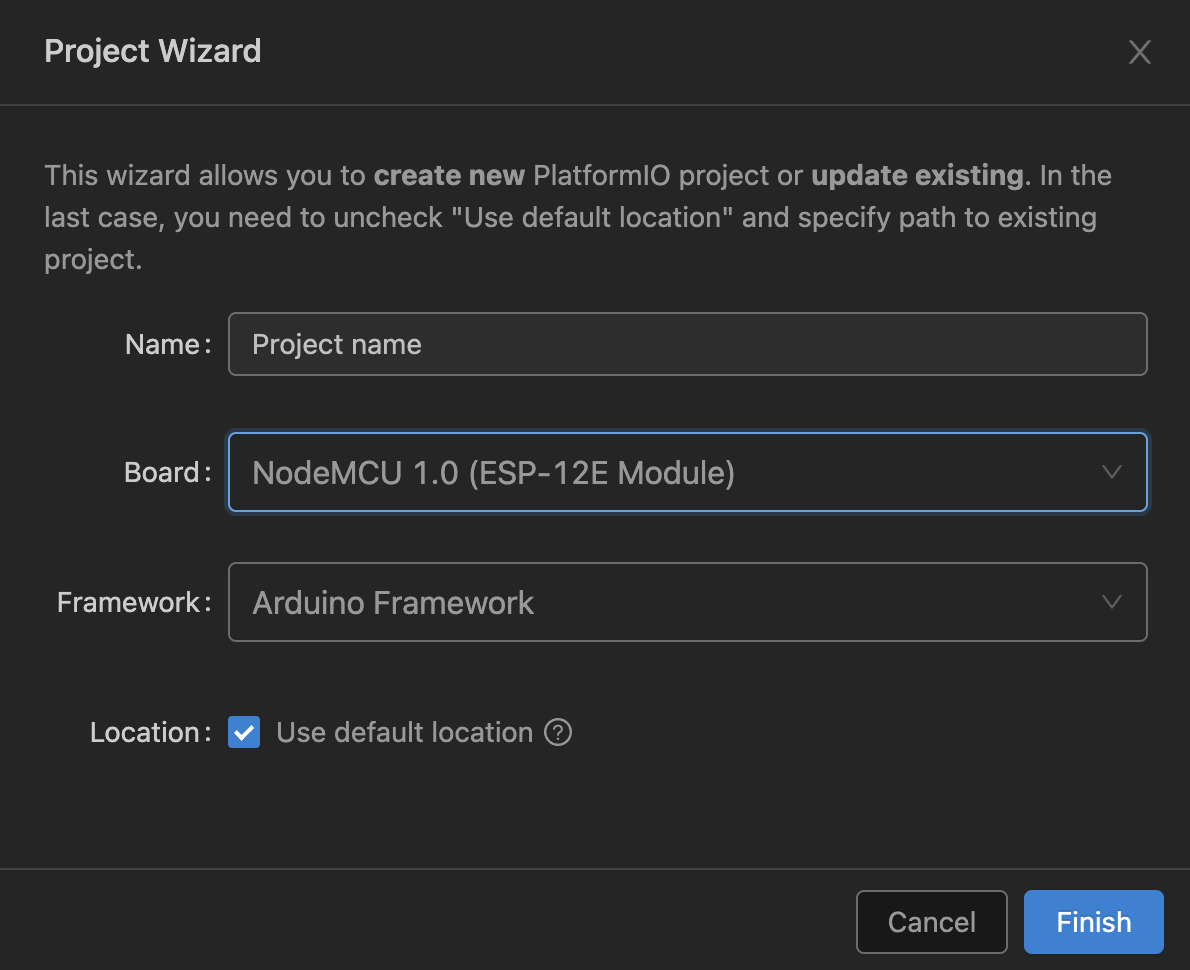
\includegraphics[scale=0.6]{resources/platformio-new-project}
		\caption{Меню создания нового проекта в PlatformIO}
		\label{fig4.1}
	\end{figure}
	
	Первым шагом при программировании микроконтроллера стало создание проекта при помощи PlatformIO.
	На этапе создания нового проекта появляется возможность выбора контроллера. Основными составляющими
	в проекте являются конфигурационный файл platformio.ini, в котором указывается модель контроллера,
	а также подключаемые к проекту библиотеки, и директива src, в которой должен содержаться код проекта.
	
	При первоначальной настройке в папке src содержится единственный файл main.cpp. Он включает два
	метода. Метод setup() отвечает за исходную конфигурацию контроллера, а метод loop()
	повторяется всё время, пока контроллер подключен к питанию.
	
	Для знакомства с программированием данного типа контроллеров и изучения программных методов
	было реализовано несколько базовых примеров. Первым из них было мигание встроенного на контроллере
	индикатора. Затем были построены простейшие схемы с использованием макетной платы, диода и
	нескольких проводов. Мигание встроенного индикатора было заменено миганием диода. После этого
	был реализован пример управления диода по нажатию кнопки. Наконец, был задействован Wi-Fi модуль
	для управления диодом с компьютера. Данный пример был взят за основу практического прототипа. Более
	подробно работа прототипа и все этапа обмена сообщениями будут рассмотрены позже. Но перед этим
	перейдём к криптографической части данной работы.
	
	\begin{figure}[h]
		\centering
		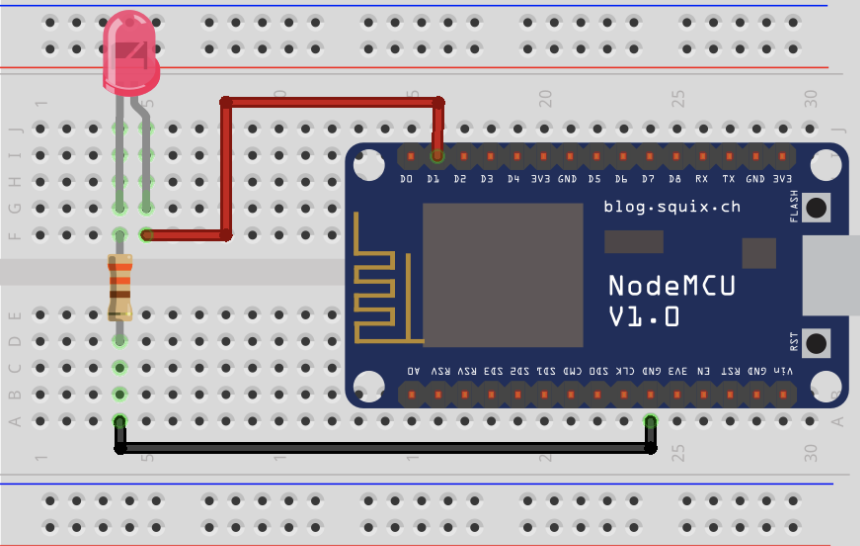
\includegraphics[scale=0.6]{resources/esp8266-control-led}
		\caption{Схема подключения диода к микроконтроллеру}
		\label{fig4.2}
	\end{figure}
	
	
	\section{Реализация и использование криптографического стандарта СТБ 34.101.77}
	
	\subsection{Описание стандарта}
	\label{standard-77-decr}
	
	Официальное название стандарта $-$ <<Криптографические алгоритмы на основе sponge-функции>> \cite{standard-77}.
	Разберём для начала, что из себя представляет sponge-функция.
	
	Sponge-функция $-$ это класс алгоритмов с конечным внутренним состоянием. Эти алгоритмы
	предназначены для обеспечения конфиденциальности, целостности и подлинности информации
	при её передачи и обработке. Сама функция задаёт сложное преобразование двоичных слов большой 
	длины. Криптографические алгоритмы подразделяются на две большие группы:
	
	\begin{enumerate}
		\item алгоритмы хэширования, описанные в разделе 7 стандарта;
		\item программируемые алгоритмы, описанные в разделе 8.
	\end{enumerate}

	В практической части данной работы используются только программируемые алгоритмы, в частности
	алгоритмы аутентифицированного шифрования, которые представляют собой последовательности 
	команд криптографического автомата. Более подробно о них речь пойдёт далее.

	Стандарт описывает преобразование двоичных слов длины 1536 бит (192 байта). Преобразование
	задаётся алгоритмом \texttt{bash-f}, который в свою очередь использует алгоритм \texttt{bash-s}. 
	Алгоритмы \texttt{bash-f} и \texttt{bash-s} определяют работу программируемых алгоритмов. Стандартные уровни
	стойкости $l = 128, 192, 256$. Дополнительным параметром является ёмкость $d \in \{1, 2\}$.
	В программируемых алгоритмах также используется ключ $K$, длина которого должна быть не меньше 
	уровня стойкости, но также не превосходить 480. Для контроля целостности и подлинности вычисляется
	имитовставка, длина которой равна уровню стойкости $l$.
	
	Управление автомата, лежащего в основе программируемых алгоритмов, осуществляется командами.
	Допустимы следующие команды:
	
	\begin{itemize}
		\item \texttt{start} (инициализация). На этом этапе происходит загрузка ключа;
		\item \texttt{restart} (повторная инициализация);
		\item \texttt{absorb} (загрузка данных);
		\item \texttt{squeeze} (выгрузка данных). С помощью этой команды осуществляется вычисление имитовставки;
		\item \texttt{encrypt} (операция зашифрования);
		\item \texttt{decrypt} (операция расшифрования);
		\item \texttt{ratchet} (необратимое изменение состояния автомата);
		\item \texttt{commit} (подтверждение выполнения других комманд).
	\end{itemize}

	В практической части данной работы были реализованы команды \texttt{start}, \texttt{absorb}, \texttt{squeeze}, \texttt{encrypt}, 
	\texttt{decrypt}, \texttt{commit}. Все перечисленные команды используются в аутентифицированном шифровании,
	которое и применяется для защиты данных, передаваемых между умными устройствами. Алгоритм
	установки защиты заключается в последовательном применении команд \texttt{start}, \texttt{absorb}, \texttt{encrypt}, \texttt{squeeze},
	а алгоритм снятия защиты выполняет команды \texttt{start}, \texttt{absorb}, \texttt{decrypt} и \texttt{squeeze} соотвественно.
	
	Алгоритмы комманд более подробно можно изучить в стандарте \cite{standard-77}, а их реализации
	на языках программирования Java и С++ приведены в приложениях к данной работе. Рассмотрим 
	более подробно алгоритмы установки и снятия защиты в аутентифицированном шифровании. В обоих
	алгоритмах используется автомат $\alpha$.
	
	\noindent\rule{\textwidth}{1pt}
	
	\textbf{Алгоритм установки защиты \texttt{bash-prg-ae}}

	\noindent\rule{\textwidth}{1pt}
	
	\textit{Вход:}
	
	\begin{itemize}
		\item $l \in \{128, 192, 256\}$, $d \in \{1, 2\}$ --- уровень стойкости и ёмкость;
		\item $A \in \{0, 1\}^{32*}$ --- анонс;
		\item $X \in \{0, 1\}^{8*}$ --- биты сообщения, которое необходимо зашифровать;
		\item $I \in \{0, 1\}^{8*}$ --- ассоциированные данные;
		\item $K \in \{0, 1\}^{32*}$ --- ключ шифрования.
	\end{itemize}
	
	\textit{Выход:}
	
	\begin{itemize}
		\item $Y \in \{0, 1\}^{|X|}$ --- биты зашифрованного сообщения;
		\item $T \in \{0, 1\}^l$ --- имитовставка.
	\end{itemize}
	
	\textit{Шаги:}
	
	\begin{enumerate}
		\item Выполнить $\alpha .start \left[l, d\right] \left(A, K\right)$;
		\item $\alpha .absorb \left(I\right)$;
		\item $Y \leftarrow \alpha .encrypt \left(X\right)$;
		\item $T \leftarrow \alpha .squeeze \left(l\right)$;
		\item возвратить $\left(Y, T\right)$.
	\end{enumerate}
	
	\noindent\rule{\textwidth}{1pt}
	
	\noindent\rule{\textwidth}{1pt}
	
	\textbf{Алгоритм снятия защиты \texttt{bash-prg-ae}$^{-1}$}
	
	\noindent\rule{\textwidth}{1pt}
	
	\textit{Вход:}
	
	\begin{itemize}
		\item $l \in \{128, 192, 256\}$, $d \in \{1, 2\}$ --- уровень стойкости и ёмкость;
		\item $A \in \{0, 1\}^{32*}$ --- анонс;
		\item $Y \in \{0, 1\}^{|X|}$ --- биты зашифрованного сообщения;
		\item $I \in \{0, 1\}^{8*}$ --- ассоциированные данные;
		\item $T \in \{0, 1\}^l$ --- имитовставка.
		\item $K \in \{0, 1\}^{32*}$ --- ключ шифрования.
	\end{itemize}
	
	\textit{Выход:}
	
	\begin{itemize}
		\item $X \in \{0, 1\}^{8*}$ --- биты расшифрованного сообщения, либо сообщение об ошибке $\bot$,
		которое означает нарушение целостности входных данных.
	\end{itemize}
	
	\textit{Шаги:}
	
	\begin{enumerate}
		\item Выполнить $\alpha .start \left[l, d\right] \left(A, K\right)$;
		\item $\alpha .absorb \left(I\right)$;
		\item $X \leftarrow \alpha .decrypt \left(Y\right)$;
		\item если $T \neq \alpha .squeeze \left(l\right)$, то возвратить $\bot$;
		\item возвратить $X$.
	\end{enumerate}
	
	\noindent\rule{\textwidth}{1pt}
	
	\subsection{Практическая реализация}
	
	Алгоритмы \texttt{bash-s} и \texttt{bash-f} являются низкоуровневыми, поскольку оперируют с битами. Поэтому они 
	были реализованы на языке программирования C. Так как язык прошивки микроконтроллера $-$ C++,
	а язык клиентского приложения $-$ Java, команды для управления автоматом при аутентифицированном 
	шифровании необходимо было реализовать на двух этих языках. Рассмотрим сначала реализацию на Java.
	
	Практически во всех командах используется алгоритм \texttt{bash-f}, в связи с чем возникла необходимость
	вызова нативного C кода из программы на Java. Для этого используется технология JNI (Java 
	Native Interface). Однако перед этим необходимо скомпилировать код на C в динамическую библиотеку.
	Рассмотрим более детально шаги для вызова нативного кода из программы на Java:
	
	\begin{enumerate}
		\item Для начала нужно создать Java класс с методом, объявленным как native:
		\begin{lstlisting}
class LibraryNative {
	public static native byte[] bash_f(byte[] array);
}
		\end{lstlisting}
		\item После этого скомпилировать файл с опцией -h для генерация header-файла:
		\begin{lstlisting}[language=Bash]
javac LibraryNative.java -h .
		\end{lstlisting}
		\item Создать файл LibraryNative.c. Скопировать определение метода из файла LibraryNative.h
		и добавить реализацию:
		\begin{lstlisting}[language=C]
#include <jni.h>
#include <inttypes.h>
#include <string.h>
#include "LibraryNative.h"

JNIEXPORT jbyteArray JNICALL Java_LibraryNative_bash_1f(JNIEnv *env, jclass thisClass, jbyteArray inJNIArray) {
	// insert implementation here
}
		\end{lstlisting}
		\item Сгенерировать динамическую библиотеку. Практическая часть данной работы выполнены на 
		операционной системе MacOS, поэтому генерируется файл с расширением .dylib:
		\begin{lstlisting}[language=Bash]
gcc -I"$JAVA_HOME/include" -I"$JAVA_HOME/inc lude/darwin" -dynamiclib -o libLibraryNative.dylib LibraryNative.c
		\end{lstlisting}
		\item Запустить метод из программы на Java, предварительно загрузив библиотеку в явном виде:
		\begin{lstlisting}
public class Runner {
	
	static {
		System.loadLibrary("LibraryNative");
	}

	public static void main(String[] args) {
		LibraryNative.bash_f(new byte[192]);
	}
}
		\end{lstlisting}
	\end{enumerate}

	Далее были реализованы команды, а также методы для установки и снятия защиты в аутентифицированном 
	шифровании строго в соответствии со стандартом.
	
	Реализация стандарта на C, как и других белорусских криптографических стандартов, содержится 
	в библиотеке bee2. Проблема заключается в несовместимости этой библиотеки с платформой PlatformIO,
	на базе которой написана прошивка для микроконтроллера. В связи с этим возникла необходимость
	реализовать часть стандарта, ответственную за шифрование, самостоятельно. За основу была взята
	имплементация из библиотеки bee2.
	
	Также в коде были реализованы юнит-тесты с данными из приложения А соответствующего стандарта для
	верификации корректности реализации алгоритмов и команд.

	
	\section{Модель прототипа}
	
	Результатом работы над практической частью является реализация протокола взаимодействия между
	двумя устройствами с применением белорусского криптографического стандарта. Протокол
	включает в себя защищённый обмен сообщениями. Рассмотрим более детально взаимодействие конечного
	устройства (умной лампочки на базе микроконтроллера ESP8266) и управляющего устройства (компьютера).
	
	На этапе присоединения конечное устройство подключается к сети Wi-Fi, в которой уже находится
	управляющее устройство. После этого на конечном устройстве запускается упрощённый веб-сервер
	(с выделенным статическим IP адресом),
	который ожидает команды от управляющего устройства. Клиент посылает HTTP POST запросы на
	включение или выключение лампочки по REST API. При этом конечное устройство принимает только 
	корректно зашифрованные запросы и не реагирует на все остальные.
	
	Рассмотрим ключевые технические особенности, которые были применены при разработке прототипа.
	
	\subsection{Распределение ключей шифрования}
	
	Основной проблемой при подключении любого умного устройства является распределение ключей
	шифрования. В практической части данной работы этот процесс осуществляется по аналогии с последней
	версией протокола ZigBee. Каждое конечное устройство имеет свой уникальный ключ шифрования.
	Предполагается наносить закодированный ключ на корпус устройства в виде QR-кода. При первом подключении
	устройства необходимо считать QR-код смартфоном и передать его на компьютер. Так управляющее
	устройство узнаёт о ключе.
	
	\begin{figure}[H]
		\centering
		
\includegraphics[scale=0.15]{resources/private-key}
		\caption{Пример QR-кода, содержащего исходный ключ шифрования}
		\label{fig4.3}
	\end{figure}

	После этого компьютер генерирует новый ключ шифрования, зашифровывает его на исходном ключе
	и отправляет на устройство в своём первом сообщении. Новый ключ записывается в память устройства
	и используется для дальнейшего обмена сообщениями. Таким образом, для каждой пары 
	<<управляющее устройство $-$ конечное устройство>> ключ шифрования является уникальным.
	
	\subsection{Установка Wi-Fi соединения}
	
	Вторым важным моментом является подключение умного устройства к нужной Wi-Fi сети. Для этого
	используется специализированная библиотека WiFiManager. Процесс подключения происходит по 
	следующей схеме:
	
	\begin{enumerate}
		\item При запуске Wi-Fi модуль на микроконтроллере работает в режиме программной точки доступа
		с предварительно заданным именем сети и паролем.
		\item На управляющем устройстве (компьютере) необходимо подключиться к соответствующей Wi-Fi сети, 
		после чего откроется страница со всеми доступными Wi-Fi сетями.
		\item В списке необходимо выбрать нужную сеть и ввести пароль.
		\item С этого момента умное устройство будет находиться в выбранной сети в качестве Wi-Fi клиента.
	\end{enumerate}
	
	Описанные действия необходимо осуществить единожды $-$ при первом подключении устройства в сеть.
	В дальнейшем контроллер будет подключаться к сети автоматически при её наличии в зоне доступа.
	
	\begin{figure}[H]
		\centering
		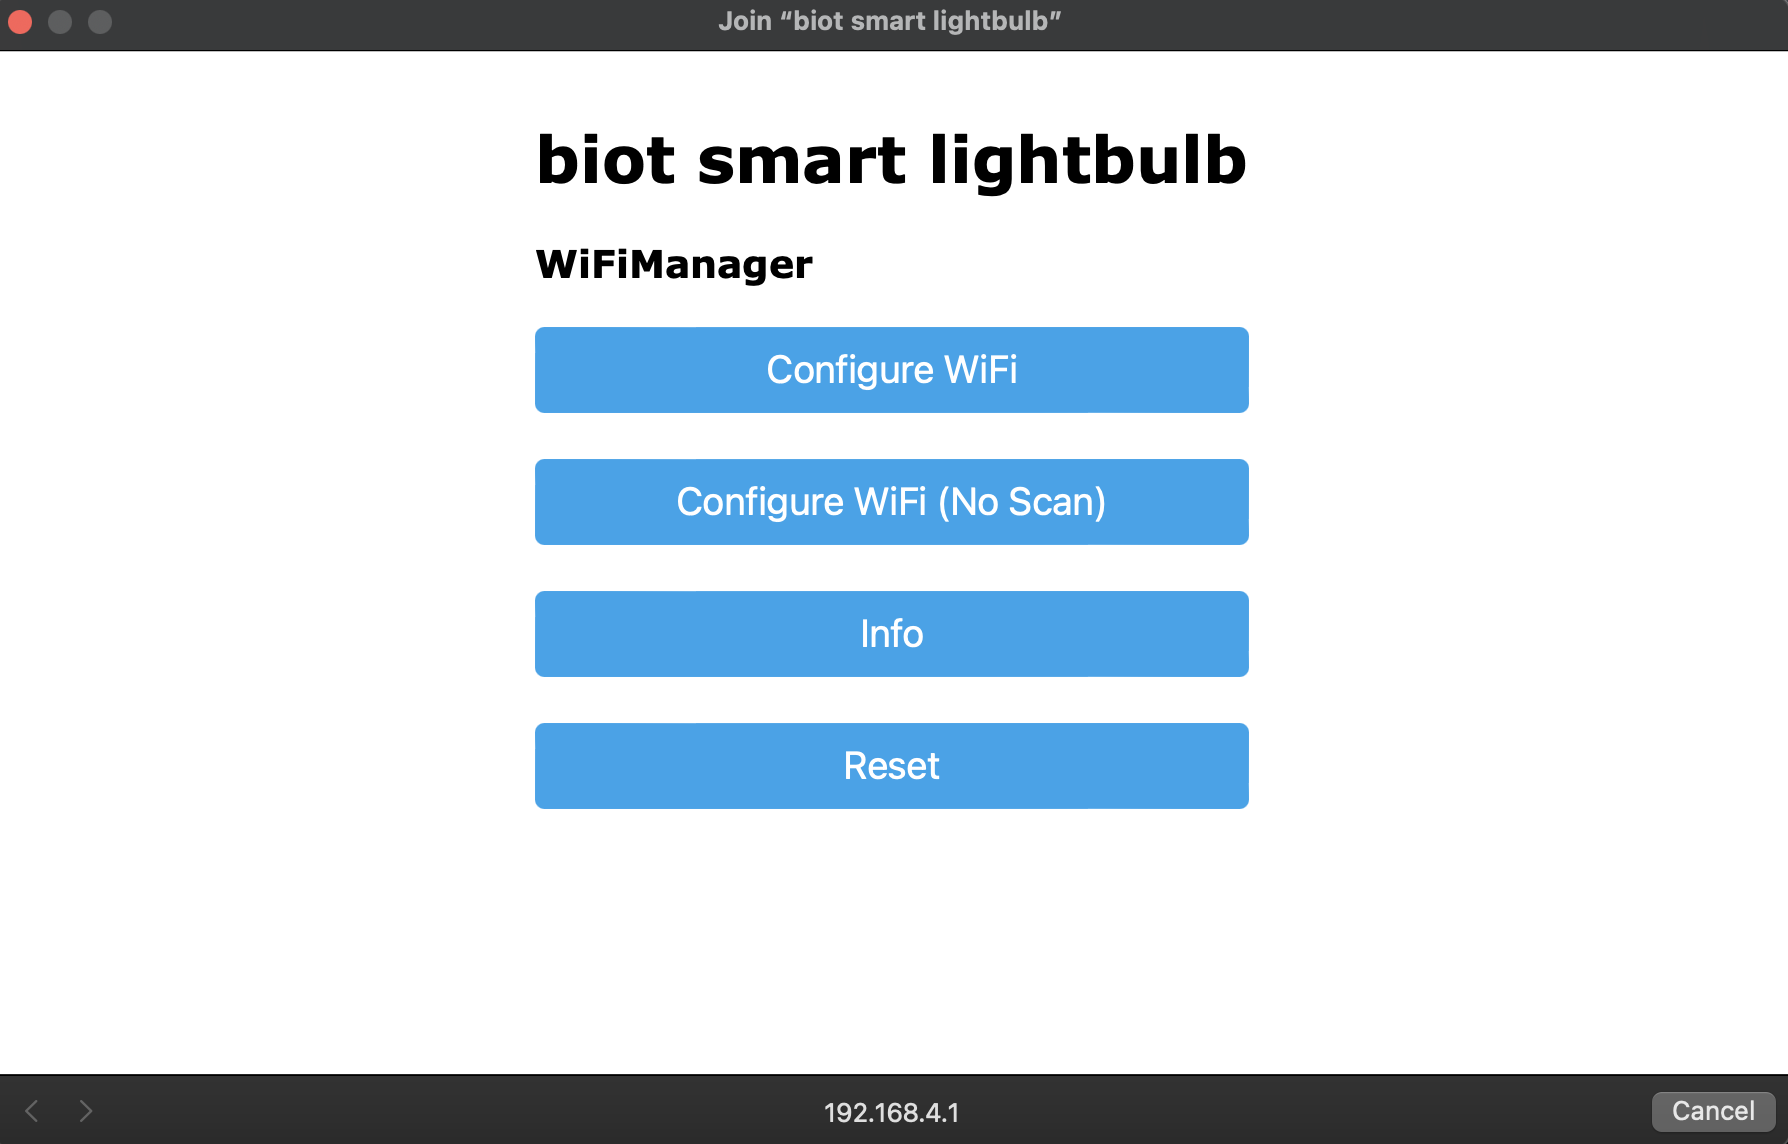
\includegraphics[scale=0.5]{resources/wifi-manager-1}
		\caption{Меню подключения умного устройства к Wi-Fi сети}
		\label{fig4.4}
	\end{figure}
	
	\subsection{Счётчик сообщений}
	
	Не менее важным механизмом является счётчик отправленных и полученных сообщений. И управляющее,
	и конечное устройства хранят в своей памяти счётчик. При первом подключении умного устройства
	счётчик равен нулю. Затем в процессе отправки сообщений после каждого сообщения (отправленного
	или полученного) счётчик увеличивается на единицу. Таким образом, после одного полного цикла
	обмена сообщениями (команда от управляющего устройства и ответ от лампочки) счётчик увеличивается
	на два.
	
	Счётчик используется в качестве синхропосылки при зашифровании и расшифровании сообщений и решает
	сразу две ключевые проблемы:
	
	\begin{enumerate}
		\item Поскольку счётчик используется при расшифровании, то при несовпадении значения счётчика 
		лампочка отбросит некорректное сообщение, а счётчик вернётся к предыдущему значению. Это обеспечивает 
		защиту от атаки повторного воспроизведения $-$ одной из базовых криптографических атак, упомянутой ранее 
		при рассмотрении матрицы угроз.
		\item Счётчик обеспечивает уникальность зашифрованных данных. Несмотря на то, что в основной часте
		работы протокола управляющее устройство отправлет две команды (на включение или выключения лампочки),
		злоумышленник при перехвате данных будет видеть каждый раз новые сообщения и не сможет установить
		никаких закономерностей.
	\end{enumerate}
	
	\subsection{Этапы обмена сообщениями}
	
	Таким образом, при первом подключении нового устройства необходимо считать с него исходный ключ
	шифрования, затем сгенерировать и отправить новый ключ, а также установить корректное Wi-Fi
	соединение. Напомним ещё раз, что все описанные выше действия осуществляются однократно. После
	этого устройства переходят в основную фазу работы протокола, в которой компьютер отправляет команды
	по включению или выключению лампочки, а лампочка в свою очередь возвращает ответ с информацией
	об успешном выполнении команды или ошибкой. Полная схема работы протокола приведена на 
	рисунке \ref{fig4.5}.
	
	\begin{figure}[h]
		\centering
		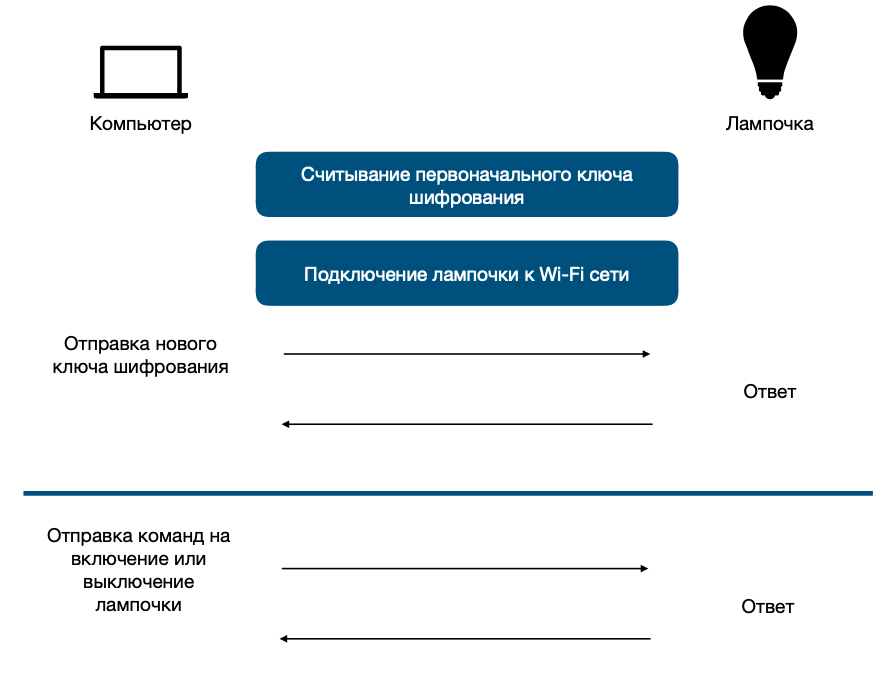
\includegraphics[scale=0.5]{resources/work-scheme}
		\caption{Этапы работы протокола}
		\label{fig4.5}
	\end{figure}

	Рассмотрим более детально основной этап работы протокола и посмотрим, что происходит с отправляемым
	сообщением на каждом шаге. Для примера возьмём команду по выключению лампочки --- сообщение \texttt{off}.
	
	\begin{enumerate}
		\item Сообщение \texttt{off} --- строка типа \texttt{String}.
		\item $\left[111, 102, 102\right]$ --- массив байт, который извлекается с помощью метода \texttt{getBytes()}.
		\item $\left[24, -88, -31\right]$ --- зашифрованный массив байт, получающийся после выполнения
		алгоритма \texttt{bash-prg-ae} (схема алгоритма рассмотрена в разделе \ref{standard-77-decr}).
		
		\small{Параллельно с этим вычисляется имитовставка $T$ --- массив фиксированной длины, состоящий из $l / 8$ байт.}
		\normalsize
		
		\item Строка \texttt{18A8E1} --- шестнадцатеричное представление зашифрованного массива байт.
		\item Строка \texttt{MThBOEUx} --- закодированная строка из предыдущего шага в формате Base64.
		В таком формате зашифрованная команда вместе с закодированной имитовставкой отправлются от управляющего
		устройства на контроллер, после чего на контроллере происходит выполнение обратных операций.
		\item Строка \texttt{18A8E1} $\rightarrow$ зашифрованный массив байт $\left[24, -88, -31\right]$
		$\rightarrow$ расшифрованный массив байт $\left[111, 102, 102\right]$ $\rightarrow$ сравнение 
		имитовставок $\rightarrow$ строка \texttt{off}. После этого лампочка распознаёт поддерживаемую
		команду, производит её выполнение и отправляет ответ клиенту с кодом сообщения 200.
		В случае же ошибки код сообщения будет 500.
	\end{enumerate}
	
	\subsection{Демонстрация работы прототипа}
	
	Для клиента было разработано веб-приложение, отображающее текущее состояние лампочки и позволяющее
	изменять его.

	При изменении положения переключателя лампочка меняет своё состояние. Прототип умного устройства
	состоит из диода, имитирующего лампочку, микроконтроллера, макетной платы и нескольких проводов,
	соединяющих всё в единое целое. Прототип получает питание через кабель от компьютера или внешнего
	аккумулятора.
	
	\begin{figure}[h]
		\centering
		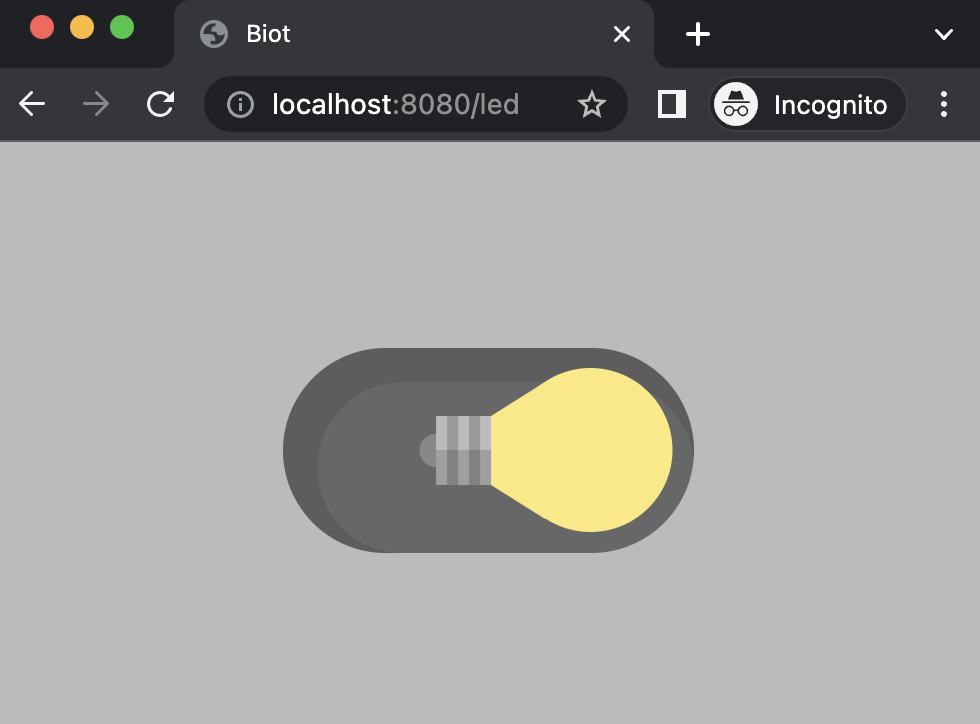
\includegraphics[scale=0.7]{resources/client-light-on}
		\caption{Интерфейс веб-приложения}
		\label{fig4.6}
	\end{figure}
	
	\begin{figure}[h]
		\centering
		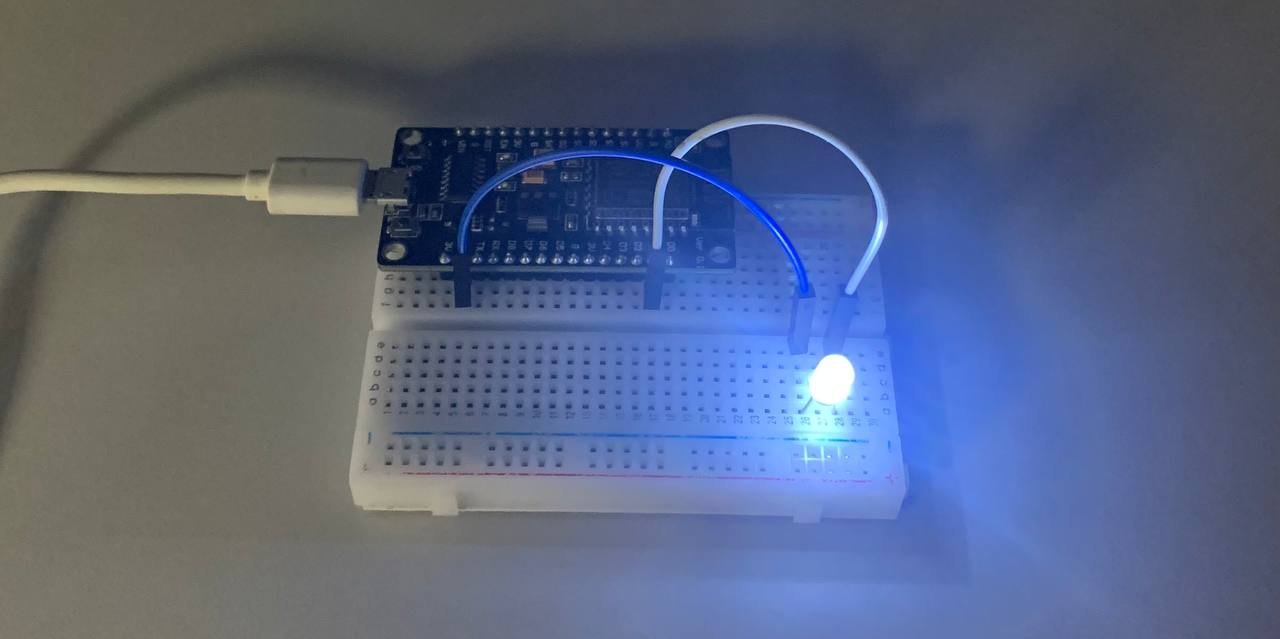
\includegraphics[scale=0.3]{resources/device-prototype}
		\caption{Прототип умной лампочки}
		\label{fig4.7}
	\end{figure}

	Для демонстрации работы шифрования был проведён эксперимент с перехватыванием данных, отправляемых
	от компьютера к лампочке по Wi-Fi сети. Для осуществление эксперимента использовался анализатор трафика
	Wireshark. На рисунке \ref{fig4.8} приведён пример незашифрованной команды по выключению лампочки,
	а на рисунке \ref{fig4.9} $-$ пример этой же команды, но уже в зашифрованном виде.
	
	\begin{figure}[H]
		\centering
		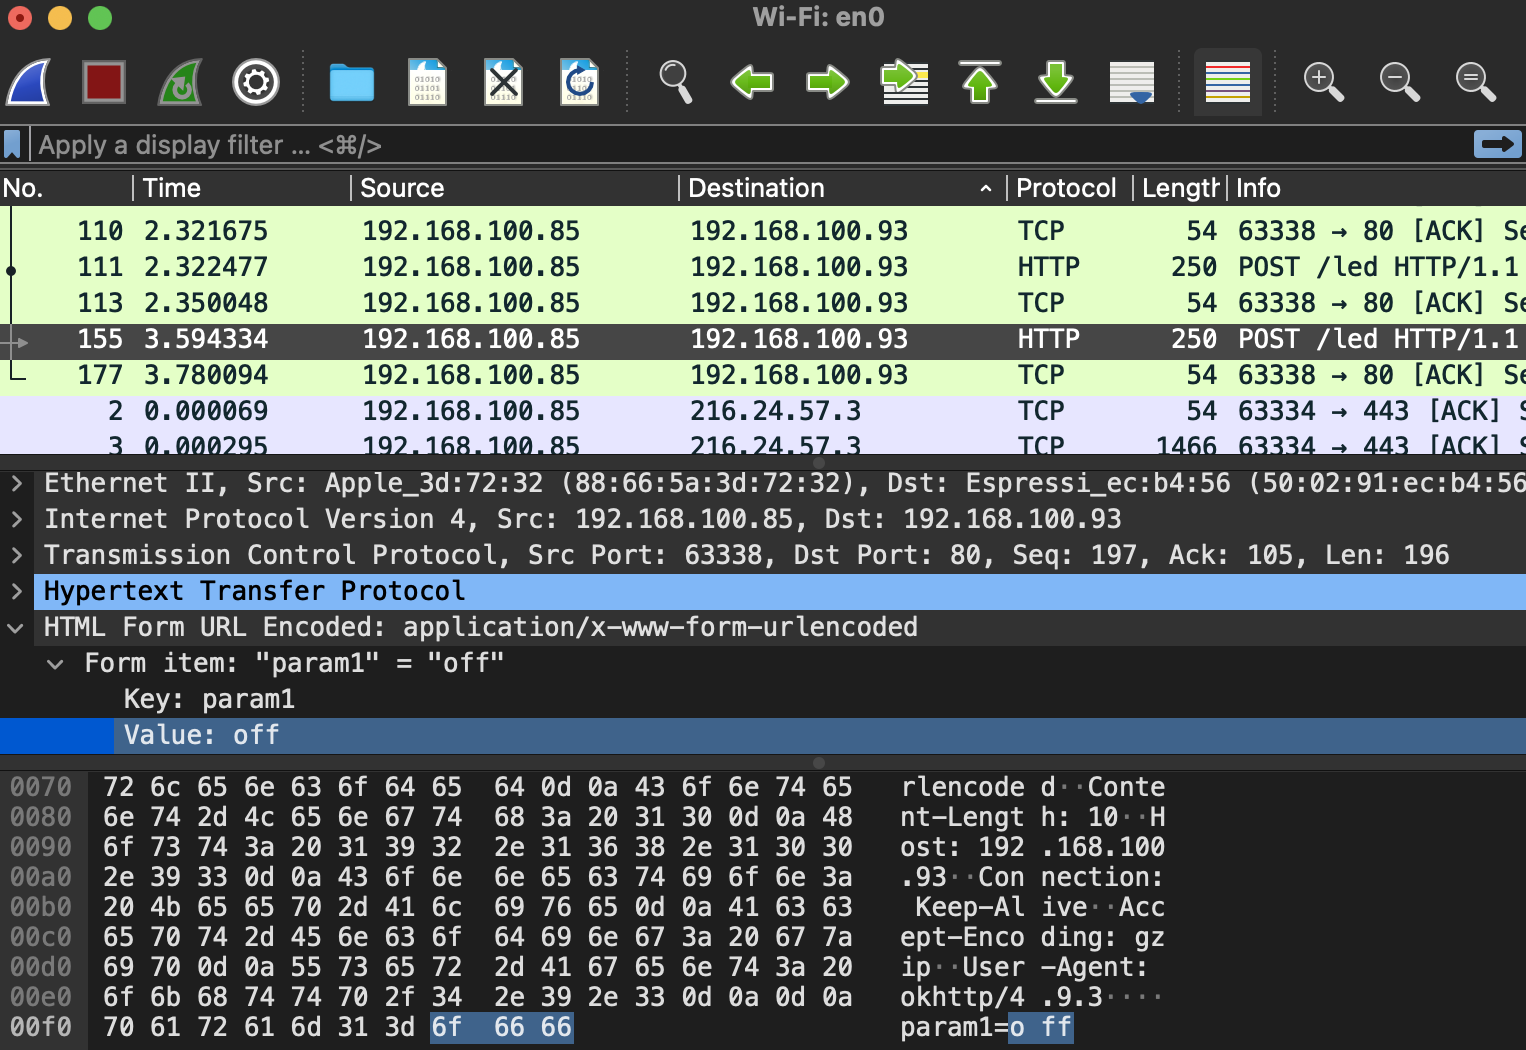
\includegraphics[scale=0.6]{resources/wireshark-encryption-disabled}
		\caption{Пример незашифрованной команды}
		\label{fig4.8}
	\end{figure}

	\begin{figure}[H]
		\centering
		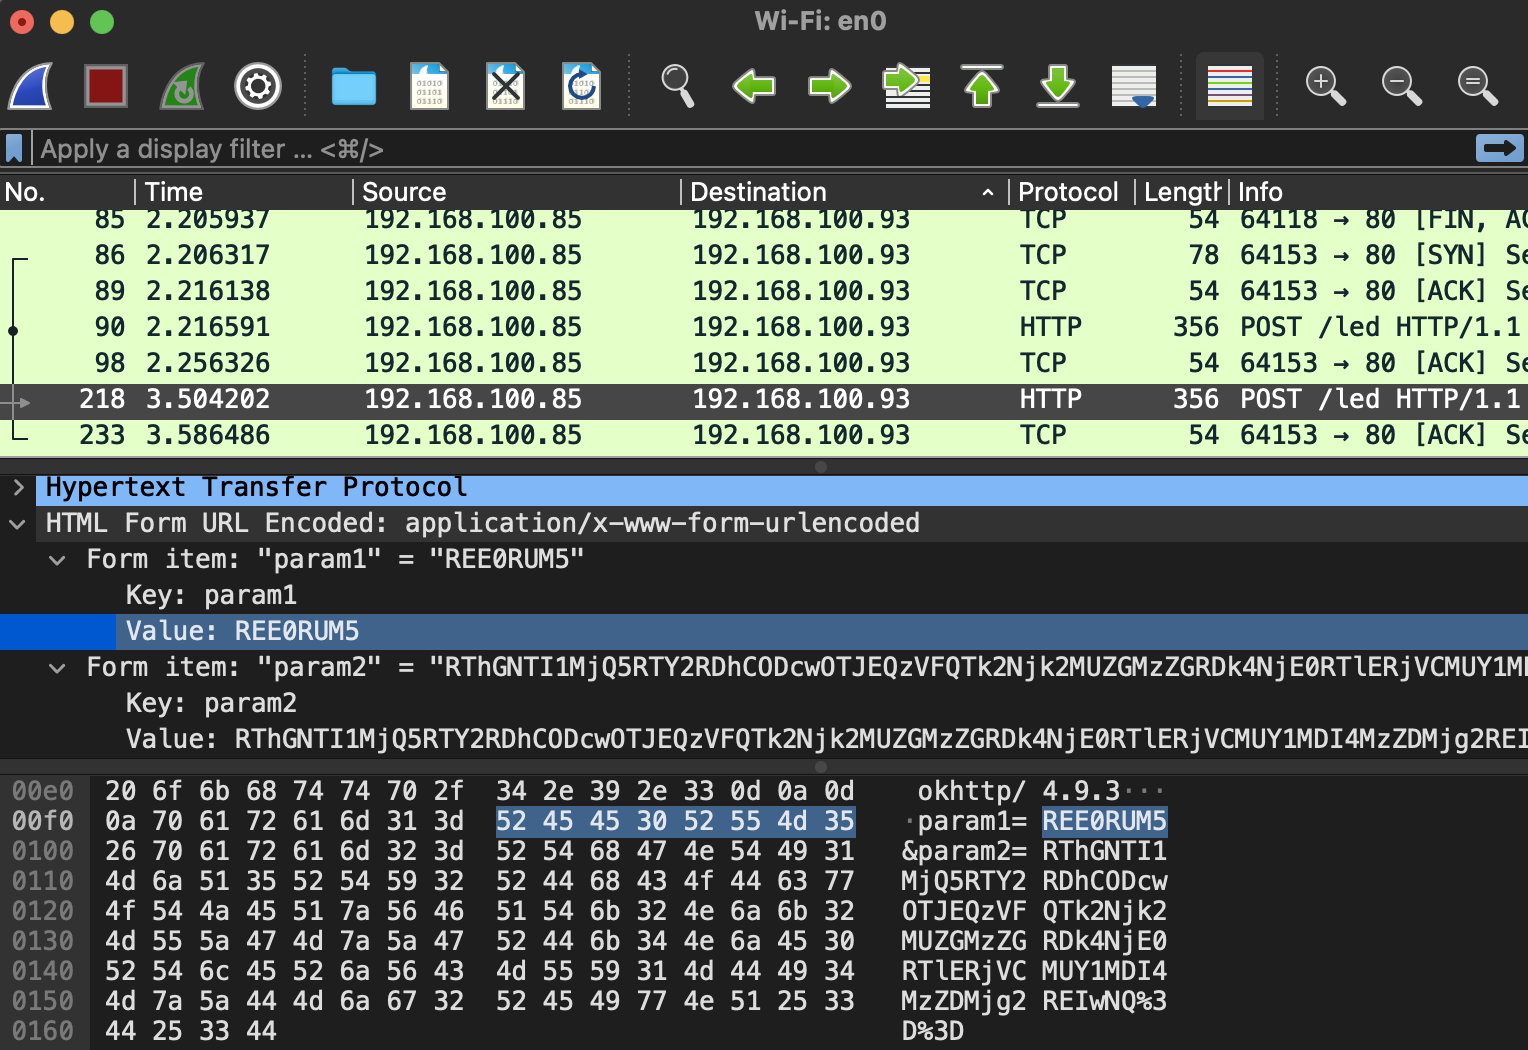
\includegraphics[scale=0.6]{resources/wireshark-encryption-enabled}
		\caption{Пример зашифрованной команды}
		\label{fig4.9}
	\end{figure}


	\section{Оценка скорости работы протокола}
	
	Для оценка скорости работы протокола была разработана небольшая утилита, способная замерять
	время работы как отдельных операций, так и этапов выполнения протокола.
	
	На рисунке \ref{fig4.10} представлен график зависимости времени выполнения 1000 операций
	зашифрования и расшифрования от длины входного сообщения. Время работы представлено
	в миллисекундах, а длина сообщения $-$ в байтах.
	
	\begin{figure}[h]
		\centering
		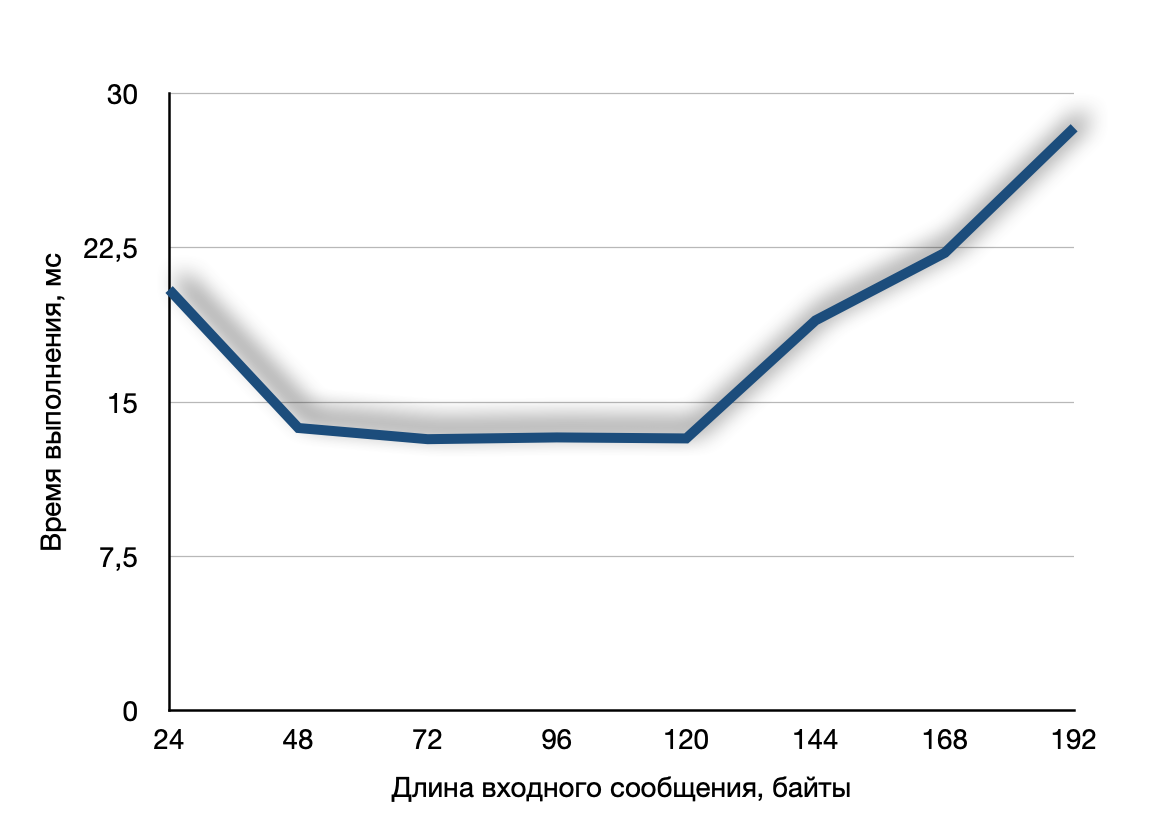
\includegraphics[scale=0.7]{resources/chart-1}
		\caption{Скорость работы операций зашифрования и расшифрования}
		\label{fig4.10}
	\end{figure}

	На рисунке \ref{fig4.11} представлен график зависимости времени выполнения полного цикла
	основного этапа работы протокола (отправка команды на включение лампочки $\rightarrow$
	ответ контроллера $\rightarrow$ отправка команды на выключение лампочки $\rightarrow$
	ответ контроллера) от размера пересылаемого сообщения. Как и на предыдущем рисунке,
	время работы представлено в миллисекундах, а длина сообщения $-$ в байтах.

	\begin{figure}[H]
		\centering
		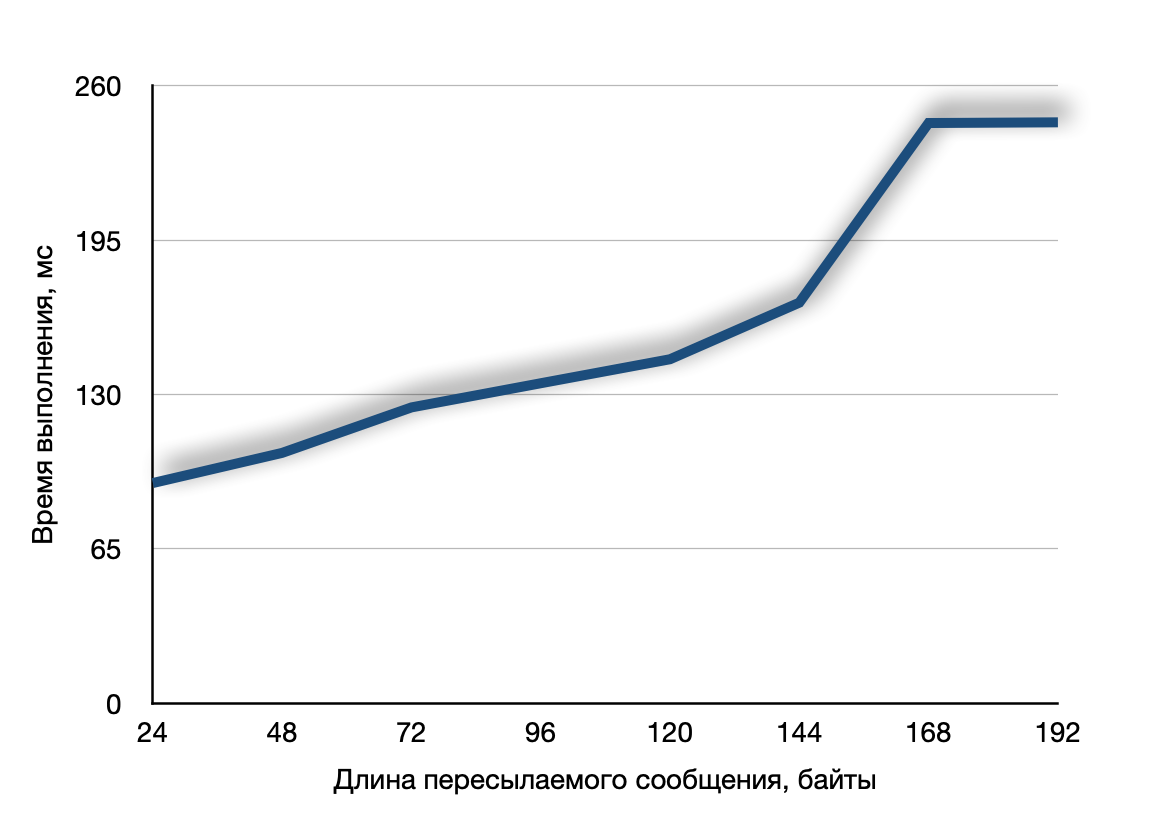
\includegraphics[scale=0.7]{resources/chart-2}
		\caption{Скорость работы протокола}
		\label{fig4.11}
	\end{figure}

	Исходя из графиков, можно сделать вывод, что зависимость между временем работы операций зашифрования 
	и расшифрования (как и временем работы всего протокола) и размером шифруемого (и пересылаемого) 
	сообщения близка к линейной.
	
	